\newgeometry{
    a4paper,
    top=24mm,
    bottom=28mm,
    left=39mm,
    right=39mm,
    heightrounded
}
\partpage{Elettrodinamica}
\restoregeometry


\chapter{Legge di Faraday}

Le prime osservazione quantitative sulle relazioni fra campi elettrici e magnetici dipendenti dal tempo furono eseguite da Faraday (1831) mediante esperimenti sul comportamento delle correnti in circuiti immersi in campo magnetici variabili nel tempo. \\

Faraday osservò che si generano delle correnti transitorie nei segenti casi:

\begin{itemize}
    \item quando in un circuito adiacente viene accesa o spenta una corrente
    \item quando il circuito adiacente, con corrente costante, viene spostato rispetto al circuito in esame
    \item quando un magnete permanente viene avvicinato o allontanato rispetto al circuito in esame
\end{itemize}

Faraday attribuì la causa della corrente transitoria in tutti e tre i casi alla \emph{variazione del flusso magnetico concatenato al circuito in esame}: la variazione del flusso induce nel circuito un campo elettrico, la cui circuitazione viene chiamata forza elettromotrice indotta $\mathcal{E}$. \mkeyword{forza elettromotrice indotta}\\

Esprimiamo ora i risultati delle osservazioni di Faraday in forma matematica. Consideriamo un superficie $\Sigma$, con versore ortogonale $\mathbf{u}_n$, che abbia il circuito $C$ come contorno. Sia $\mathbf{B}$ il campo magnetico nella regione occupata dal circuito; il flusso magnetico concatenato è definito dalla formula:

\begin{equation}
\Phi (\mathbf{B}) = \int_{\Sigma} \mathbf{B} \cdot \mathbf{u}_n \, d\Sigma
\end{equation}

La forza elettromotrice lungo il circuito è definta come 

\begin{equation}
    \mathcal{E} = \oint_C \mathbf{E'} \cdot d\mathbf{l}
\end{equation}

dove $\mathbf{E}'$ è il campo elettrico indotto in corrispondenza dell'elemento $d \mathbf{l}$ di $C$. \\

I risultati delle osservazioni di Faraday sono riassunti nella forma

\begin{tcolorbox}[colback=yellow!10!white, colframe=orange!70!black, boxrule=0.8pt]
\begin{equation} \label{eq: Legge di Faraday}
\mathcal{E} = -\frac{d\Phi (\mathbf{B})}{dt}
\end{equation}
\end{tcolorbox}

Questa relazione prende il nome di \emph{Legge di Faraday}. \mkeyword{Legge di Faraday} \\

\newpage

\subsection{Legge di Lenz}

Il segno meno che compare nella \ref{eq: Legge di Faraday} è molto importante e viene messo in evidenza con un enunciato particolare, detto \emph{legge di Lenz}: l'effetto della forza elettromotrice indotta è sempre tale da opporsi alla causa che ha generato il fenomeno. \\

Ad esempio, se in un circuito chiuso circola una corrente indotta, questa ha verso tale che il flusso del proprio campo magnetico concatenato col circuito si oppone alla variazione del flusso primario $\Phi$.\\

Questo comportamento è in accordo con il principio di conservazione dell'energia. 

\section{Invarianza sotto trasformazioni di Galileo}

Prima dello sviluppo della relatività speciale (e anche dopo, nei casi in cui si ha a che fare con velocità relative piccole rispetto alla velocità della luce) tutti i fisici erano concordi nel ritenere che tutte le leggi fisiche dovessero essere invarianti rispetto a trasformazioni di Galieleo. \\

Ciò significa che tutti i fenomeni fisici devono apparire identici a due osservatori che si muovono l'uno rispetto all'altro con velocità relativa $\mathbf{v}$ costante.\\

Consideriamo ora la legge di Faraday per un circuito (secondario) in moto e vediamo le conseguenze dell'invarianza galileiana. \\
Esprimendo la \ref{eq: Legge di Faraday} madiante integrali dei campo $\mathbf{E}'$ e $\mathbf{B}$, si ha 

\begin{equation} \label{eq: L. Faraday integrale}
    \oint_C \mathbf{E'} \cdot d \mathbf{l} = - \int_{\Sigma} \mathbf{B} \cdot \mathbf{u}_n \ d\Sigma
\end{equation}

La linea di integrazione può essere pensata come una linea geometrica chiusa qualsiasi, non necessariamente materializzata da un filo conduttore, e la \ref{eq: Legge di Faraday} diventa così una relazione generale fra i campi. \\

\' E tuttavia importante notare che il campo elettrico $\mathbf{E}'$ è il campo elettrico nel punto in cui si trova l'elemento $d \mathbf{l}$, misurato nel sistema di coordinate in cui $d \mathbf{l}$ è in quiete.\\

Se il circuito $C$ si muove con velocità $\mathbf{v}$ in un certa direzione, la derivata temporale totale che compare nella \ref{eq: Legge di Faraday} deve tener conto anche di questo movimento. 

\begin{figure} [h]
    \centering
    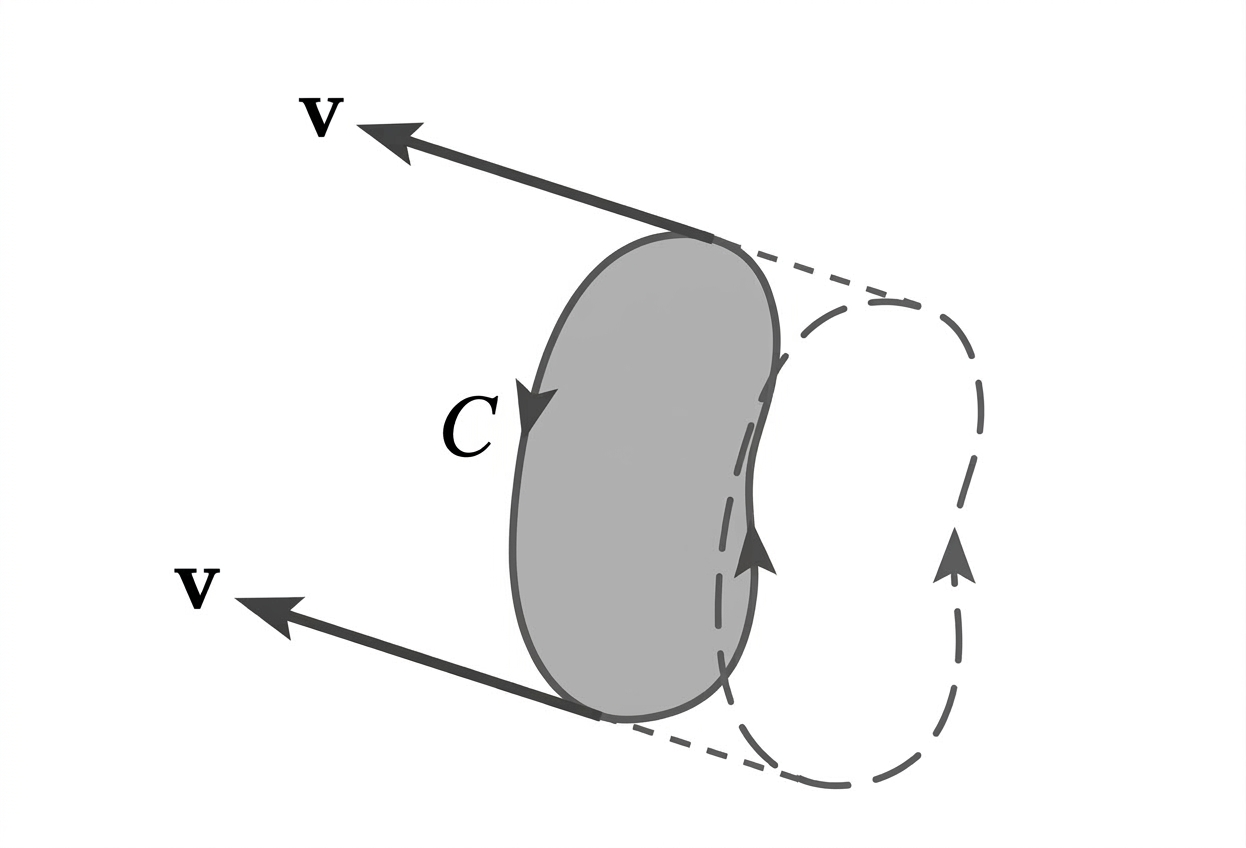
\includegraphics[width=0.4\linewidth]{figure/image63.png}
    \caption{}
\end{figure}

Il flusso concatenato nel sistema può variare perché:

\begin{itemize}
    \item varia col tempo il valore di $\mathbf{B}$ in tutti o in qualche punto.
    \item il movimento del circuito fa cambiare nel tempo la posizione del contorno. 
\end{itemize}

\newpage

\' E facile dimostrare che la derivata temporale totale del flusso concatenato si può scrivere nella forma 

\begin{equation}
    \frac{d}{dt} \int_{\Sigma} \mathbf{B} \cdot \mathbf{u}_n \ d \Sigma = \int_{\Sigma} \frac{\partial \mathbf{B}}{\partial t} \cdot \mathbf{u}_n \ d \Sigma + \oint_C (\mathbf{B} + \mathbf{v}) \cdot d \mathbf{l}
\end{equation}

L'equazione \ref{eq: L. Faraday integrale} può essere riscritta nella forma 

\begin{equation}
    \oint_C \left[ \mathbf{E'} - (\mathbf{v} \times \mathbf{B}) \right] \cdot d \mathbf{l} = - \int_{\Sigma} \frac{\partial \mathbf{B}}{\partial t} \cdot \mathbf{u}_n \ d\Sigma
\end{equation} 

Questo non è altro che una diversa enunciazione della legge di Faraday applicata al circuito in moto $C$. Ma possiamo anche interpretarla diversamente. Possiamo considerare il circuito $C$ e la superficie $\Sigma$ come situati, ad un certo istante, in una posizione fissa rispetto al sitema del laboratorio. Apllicando la legge di Faraday \ref{eq: Legge di Faraday} a questo circuito fissato, possiamo scrivere

\begin{equation}
    \oint_C \mathbf{E} \cdot d \mathbf{l} = - \int_{\Sigma} \frac{\partial \mathbf{B}}{\partial t} \cdot \mathbf{u}_n \ d\Sigma 
\end{equation}

Dove $\mathbf{E}$ è il campo elettrico misurato nel sistema del laboratorio. L'ipotesi di invarianza galileiana implica che i primi membri delle due equazioni devono essere uguali. 
Ciò significa che il campo elettrico $\mathbf{E}'$, misurato nel sistema di coordinate in moto, deve soddisfare 

\begin{tcolorbox}[colback=yellow!10!white, colframe=orange!70!black, boxrule=0.8pt]
\begin{equation} 
    \mathbf{E}' = \mathbf{E} + (\mathbf{v} \times \mathbf{B})
\end{equation}
\end{tcolorbox}

\subsection{Forma diffenziale della legge di Faraday}

Ma allora la legge di Faraday può essere posta in forma differenziale  usando il teorema di Stokes, purché il circuito cosiderato sia fisso nel sistema di riferimento scelto. Trasformando l'integrale che esprime la forza elettromotrice in un intrgrale di superficie si ottiene

\begin{equation}
    \int_{\Sigma} \left( \nabla \times \mathbf{E} + \frac{\partial \mathbf{B}}{\partial t}  \right) \cdot \mathbf{u}_n \ d\Sigma = 0
\end{equation}

Dato che il contorno $C$ e la superficie $\Sigma$ sono arbitrari, l'integrando deve essere nullo ovunque. \\

\newpage

Pertanto, la forma differenziale dell alegge di Faraday è 

\begin{tcolorbox}[colback=yellow!10!white, colframe=orange!70!black, boxrule=0.8pt]
\begin{equation} 
    \nabla \times \mathbf{E} = - \frac{\partial \mathbf{B}}{\partial t}
\end{equation}
\end{tcolorbox}

Notiamo che questa non è altro che l'estensione, al caso di campi dipendenti dal tempo, della proprietà $\nabla \times \mathbf{E} = 0$ valida per i campi elettrici statici. 

\section{Autoinduzione}

Un circuito di forma qualunque percorso da corrente produce un campo magnetico secondo la legge di Ampère-Laplace.
Il flusso di questo campo concatenato col circuito stesso, detto \emph{autoflusso} \mkeyword{autoflusso}, è dato da:

\begin{equation*}
    \Phi(\mathbf{B}) = \int_{\Sigma} \left( \oint_{C} \frac{\mu_0 i}{4 \pi} \frac{d \mathbf{s} \times \mathbf{u}_r}{r^2} \right) \cdot \mathbf{u}_n \ d\Sigma
\end{equation*}

dove $\Sigma$ è una qualunque superficie che abbia come contorno $C$. Sia il campo magnetico che, di conseguenza, il flusso del campo magnetico sono proporzionali alla corrente e si sfrutta questa proprietà per scrivere l'autoflusso come

\begin{tcolorbox}[colback=yellow!10!white, colframe=orange!70!black, boxrule=0.8pt]
\begin{equation} 
    \Phi (\mathbf{B}) = L i 
\end{equation}
\end{tcolorbox}

Il fattore $L$ si chiama coefficiente di autoinduzione o induttanza \mkeyword{induttanza} del circuito. Esso dipende dalla forma del circuito e dalle proprietà magnetiche del mezzo. 

\subsection{Forza elettromotrice di autoinduzione}

La nozione di autoflusso acquista particolare importanza quando la corrente nel circuito non è costante nel tempo oppure quando viene variata la forma del circuito. 
In entrambi i casi, come nel caso più generale in cui le due variazioni avvengano contemporaneamente, il flusso concatenato col circuito cambia nel tempo e nel circuito compare una f.e.m. indotta che con i suoi effetti tende ad opporsi alla variazione che l’ha generata. 
Tale forza elettromotrice, detta di autoinduzione, si calcola usando la \ref{eq: Legge di Faraday}:

\begin{equation}
    \mathcal{E}_L = - \frac{d \Phi}{dt} = - \frac{d}{dt} (Li)
\end{equation}

Nei casi pratici più comuni il coefficiente di autoinduzione resta costante e assume la forma

\begin{tcolorbox}[colback=yellow!10!white, colframe=orange!70!black, boxrule=0.8pt]
\begin{equation} 
    \mathcal{E}_L = - L \frac{di}{dt}
\end{equation}
\end{tcolorbox}

\newpage

\section{Mutua indunzione}

Supponiamo di considerare due circuiti, allora si definisce il flusso del campo magentico prodotto dal primo circuito attraverso il secondo come 

\begin{equation}
    \Phi_{1,2} = \int_{\Sigma_2} \mathbf{B}_1 \cdot \mathbf{u}_n \ d\Sigma_2 
\end{equation}

dove $\Sigma_2$ è una qualunque superficie che si appoggia sul secondo circuito.
Dal momemento che $B_1$ è proporzionale a $i_1$ prossiamo scrivere

\begin{tcolorbox}[colback=yellow!10!white, colframe=orange!70!black, boxrule=0.8pt]
\begin{equation}
    \Phi_{1,2} = M_{1,2} i_1
\end{equation}
\end{tcolorbox}

conglobando in $M_{1,2}$ tutti i fattori geometrici e l'eventuale dipendenza dalle proprietà magnetiche del mezzo in cui sono immersi i circuiti. \\

In modo analogo si trova che il flusso del campo magnetico del secondo circuito attraverso il primo è 

\begin{tcolorbox}[colback=yellow!10!white, colframe=orange!70!black, boxrule=0.8pt]
\begin{equation}
    \Phi_{2,1} = M_{2,1} i_2
\end{equation}
\end{tcolorbox}

Un risultato molto importante (che però non andremo a dimostrare) e utile nella risoluzione di problemi è che vale l'uguaglianza 

\begin{tcolorbox}[colback=yellow!10!white, colframe=orange!70!black, boxrule=0.8pt]
\begin{equation}
    M_{1,2} = M_{2,1}
\end{equation}
\end{tcolorbox}

\subsection{Circuiti accoppiati}

Come per il fenomeno dell'autoinduzione, anche quello della mutuainduzione diventa fondamentale quando si ha variazione di corrente e quindi una variazione del flusso.\\

Supponendo che $M$ sia costante, si ha per le forze elettromotrici indotte in un circuito dallla variazione di corrente nell'altro

\begin{equation}
    \mathcal{E}_1' = - \frac{d \Phi_{2,1}}{dt} = - M \frac{di_2}{dt} \quad , \quad \mathcal{E}_2' = - \frac{d \Phi_{1,2}}{dt} = - M \frac{di_1}{dt}
\end{equation}

Queste vanno sommate in ciascun circuito alle forze elettromotrici di autoinduzione ottenendo in questo modo, applicando la seconda legge di Kirchoff e supponendo che in uno dei due circuiti ci sia un generatore:

\begin{tcolorbox}[colback=yellow!10!white, colframe=orange!70!black, boxrule=0.8pt]
\begin{align*}
    \mathcal{E}(t) - L_1 \frac{di_1}{dt} - M \frac{di_2}{dt} = R_1 i_1 \\
    - L_2 \frac{di_2}{dt} - M \frac{di_1}{dt} = R_2 i_2
\end{align*}
\end{tcolorbox}

Vediamo che la presenza di una corrente $i_2$ nel circuito senza generatore è possibile proprio grazie al processo di mutua induzione.

